\documentclass[acmsmall]{acmart}
\usepackage[UTF8, fontset=macnew]{ctex}
\usepackage{graphicx}
\graphicspath{ {./images/} }


%%
%% \BibTeX command to typeset BibTeX logo in the docs


%%
%% Submission ID.
%% Use this when submitting an article to a sponsored event. You'll
%% receive a unique submission ID from the organizers
%% of the event, and this ID should be used as the parameter to this command.
%%\acmSubmissionID{123-A56-BU3}

%%
%% The majority of ACM publications use numbered citations and
%% references.  The command \citestyle{authoryear} switches to the
%% "author year" style.
%%
%% If you are preparing content for an event
%% sponsored by ACM SIGGRAPH, you must use the "author year" style of
%% citations and references.
%% Uncommenting
%% the next command will enable that style.
%%\citestyle{acmauthoryear}

%%
%% end of the preamble, start of the body of the document source.
\begin{document}

%%
%% The "title" command has an optional parameter,
%% allowing the author to define a "short title" to be used in page headers.
% \title{Learn How to write a apporpriate resume by example - The preliminary text mining on the open data}
\title{透過實際案例學習如何撰寫好的求職履歷 - 使用文字探勘技術之初步研究}

%%
%% The "author" command and its associated commands are used to define
%% the authors and their affiliations.
%% Of note is the shared affiliation of the first two authors, and the
%% "authornote" and "authornotemark" commands
%% used to denote shared contribution to the research.

\author{李昀潔}
\affiliation{%
    \institution{資管博一}
}
\author{呂孟芸}
\affiliation{%
    \institution{國企四}
}
\author{張譯心}
\affiliation{%
    \institution{國企四}
}
\author{陳韋霖}
\affiliation{%
    \institution{資工碩一}
}
\author{詹雅安}
\affiliation{%
    \institution{會計四}
}

%%
%% By default, the full list of authors will be used in the page
%% headers. Often, this list is too long, and will overlap
%% other information printed in the page headers. This command allows
%% the author to define a more concise list
%% of authors' names for this purpose.
% \renewcommand{\shortauthors}{Trovato and Tobin, et al.}

%%
%% The abstract is a short summary of the work to be presented in the
%% article.
\begin{abstract}
    對於學生而言,除了努力完成學業或完成研究以取得畢業之外,
    如何透過簡歷(Resume)的撰寫去應徵企業的招募也是一件重要的事。
    然而如何撰寫簡歷不是一件簡單的。
    因此我們小組從網際網路上找尋到一個人簡歷的開放資料集,
    透過分群方法(Clustering)來對該資料集進行研究,
    我們檢驗履歷的寫法是否能對應到公司招聘的職位,
    另外我們也找出一些能夠申請多種工作類別的簡歷寫法,
    此次研究希望透過該開放資料集所作的初步研究,
    希望能對學生們製作個人簡歷上能有所幫助。
\end{abstract}

%%
%% The code below is generated by the tool at http://dl.acm.org/ccs.cfm.
%% Please copy and paste the code instead of the example below.
%%

\begin{CCSXML}
<ccs2012>
   <concept>
       <concept_id>10010405</concept_id>
       <concept_desc>Applied computing</concept_desc>
       <concept_significance>500</concept_significance>
       </concept>
   <concept>
       <concept_id>10010405.10010497</concept_id>
       <concept_desc>Applied computing~Document management and text processing</concept_desc>
       <concept_significance>500</concept_significance>
       </concept>
 </ccs2012>
\end{CCSXML}

\ccsdesc[500]{Applied computing}
\ccsdesc[500]{Applied computing~Document management and text processing}

\ccsdesc[500]{Applied computing}


%%
%% Keywords. The author(s) should pick words that accurately describe
%% the work being presented. Separate the keywords with commas.
% \keywords{datasets, neural networks, gaze detection, text tagging}

%% A "teaser" image appears between the author and affiliation
%% information and the body of the document, and typically spans the
%% page.
\iffalse
\begin{teaserfigure}
  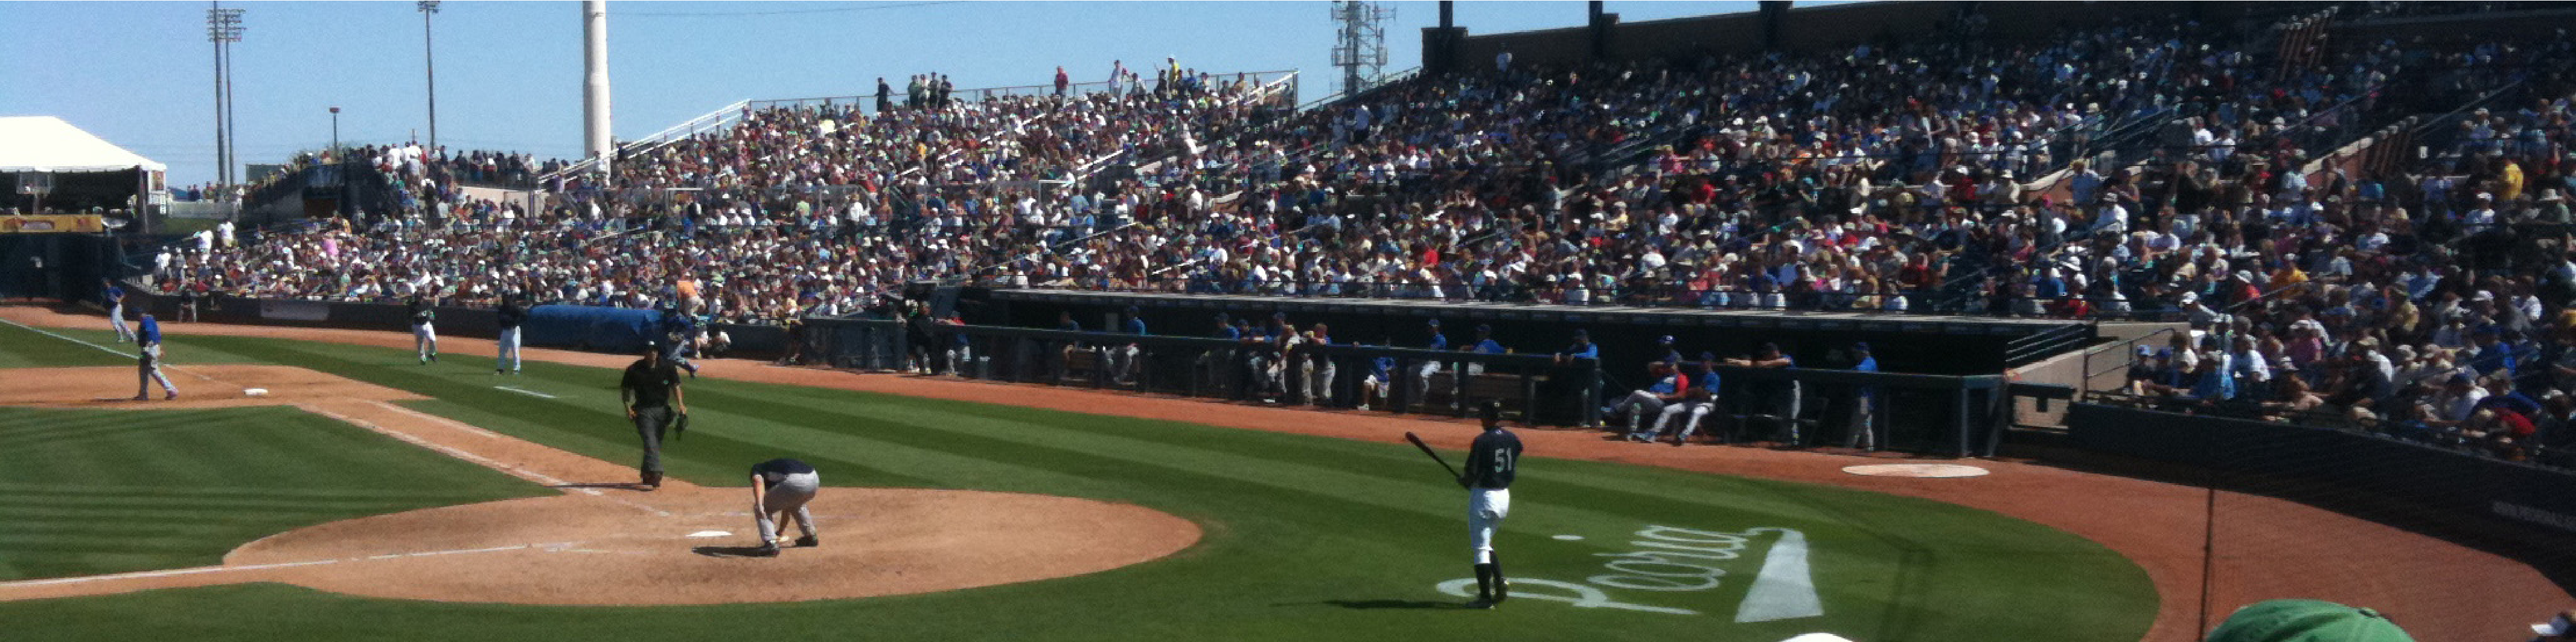
\includegraphics[width=\textwidth]{sampleteaser}
  \caption{Seattle Mariners at Spring Training, 2010.}
  \Description{Enjoying the baseball game from the third-base
  seats. Ichiro Suzuki preparing to bat.}
  \label{fig:teaser}
\end{teaserfigure}
\fi

%%
%% This command processes the author and affiliation and title
%% information and builds the first part of the formatted document.
\maketitle

\section{研究目標}

投履歷找工作時,
如何撰寫一份符合業主要求的履歷,
尤其對於高度專業的工作而言,
更顯重要,
然如何撰寫履歷等事宜,
雖坊間有許多教條方法供大眾學習,
但寫法上需考慮求職者的狀況,
並無法直接使用法則來套用。
有鑑於此,
我們使用網路上公開之求職簡歷資料,
運用課堂所學習之文字探勘技術來針對該些資料進行分析,
藉此探求有趣的訊息以幫助求職者來面對如何撰寫履歷之問題,
於本專案中,
我們設定了兩個主題進行探討,
其一為驗測該些資料是否各對應之履歷內容是否符合該求職之工作,
其二為找出部份具有跨領域寫法之履歷。

\section{研究方法}

本專案中,
我們所探討之資料,
為從網路上所抓下來之公開資料,
而該些資料除了各履歷的內容外,
也包含了各別履歷所對應之求職職位。

以文字探勘而言,
雖然求職職位與其履歷資料這兩種資料型可視為一種監督式學習技術之應用(Supervised Learning)\cite{murphy2012machine}。
然於本專案中,
欲探討之主體非以分類問題之面象而進行之,
而是希望從資料本身特性出發,
藉由資料分析方法,
試圖找出有趣的履歷範本,
意即透過非監督式學習技術(Unsupervised Learning)\cite{murphy2012machine}。

關於分析內容,
共分為兩項工作,
第一我們先檢驗資料集內容是符合常識,
意即我們想確認是否各求職類別是否對應該些求職履歷,
透過分群的方法去檢驗是否各群集(Cluster)內是否有內聚,
第二透過分析資料內容,
找出部份具有跨領域之履歷資料並作為範本供讀者參考,
其方法上我們視此該些資料視為資料探勘問題\cite{han2011data},
以找出適合之履歷資料。

\subsection{資料集}

針對履歷資料,
我使用了公開資料集作為本專案之資料,
其以Kaggle網站公開之實際之工作求職者履歷資料進行分析\cite{kaggle_dataset}。

該資料共擁有三個欄位,
分別為ID,
Resume\_str,
Resume\_html及Category,
ID欄位表示流水號,
中間兩欄位分別為Resume的純文字及其原始抓下來的格式(內含HTML標籤),
Category表示對應所求職之職位名,
此資料集共有24個求職職位,
求職種類及數量表可參照圖.~\ref{counter_of_application}。
資料集共有2484筆資料,
意即共有2484筆resume。

\begin{figure}
    \centerline{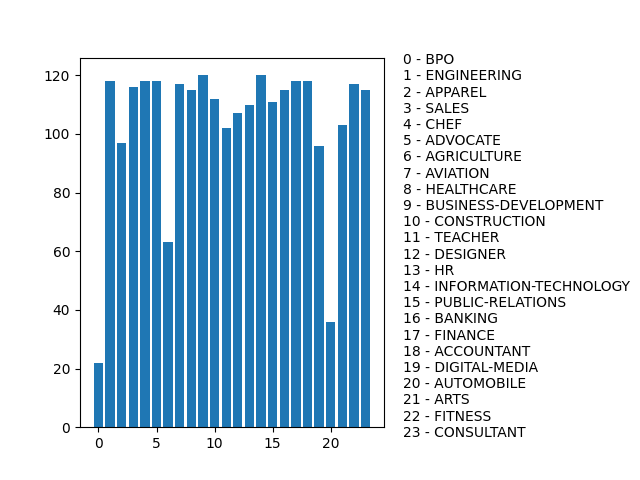
\includegraphics[width=1.0\textwidth]{counter_of_application.png}}
    \caption{The counting for each application catogery in resume}
    \label{counter_of_application}
\end{figure}

\subsection{資料前處理}

於本專案中,
我們主要進行兩項工作,
然而在進行之前,
我們需要進行資料前處理工作,
才能將履歷資料轉換成我們可以分析的資料。

我們透過使用Sentence-Transformers\cite{reimers-2020-multilingual-sentence-bert}工具,
將資料集之真實履歷資料,
透過BERT方法\cite{devlin2018bert},
將該些履歷內的文字,
轉成合適之word embeddings。
該些word embeddings為資料集中,
所有履歷之文字,
經過轉換後之新資料表示法,
其原因為,
若不經過轉換,
原始資料中所有文字所表示之方法,
其通常表示法可能為詞袋(bag of word)或是one-hot encoding編碼等,
但這些表示法都有空間浪費的問題,
因為所有文字所產生之矩陣(Matrix)都具有高度稀疏性\cite{schutze2008introduction},
因此透過BERT轉換\cite{devlin2018bert},
將原有的矩陣維度進行降維(dimension reduction),
可在保存原有資料的特徵外,
減少了原本高度稀疏所造成的問題。

\subsection{履歷一致性}

在取得word embeddings後,
我們會先針對此資料,
使用python的sklearn\cite{sklearn_api}套件,
使用主流之分群方法進行檢驗\cite{han2011data},
其目的為確保該些履歷資料具有可信性,
意即針對特定群體之履歷,
其所對應之相同職缺,
該些個別履歷資料之特性應具有相似性。

第一種分群方法,
我們採用k-means分群方法\cite{macqueen1967some},
第二種分群方法,
我們採用PCA(Princial Component Analysis)\cite{pearson1901liii}。
%第三種分群方法,
%我們採用DBSCAN(Density-based spatial clustering of applications with noise)DBSCAN\cite{ester1996density}。

針對結果,
我使用了t-sne\cite{van2008visualizing}作圖像化。


\subsection{跨領域範本}

我們使用歐及里德距離公式,
計算出各群之中存在較偏遠之履歷資料,
並將其視為具有跨領域性質之履歷。

\section{研究結果}

\subsection{履歷一致性}

\begin{figure}
    \centerline{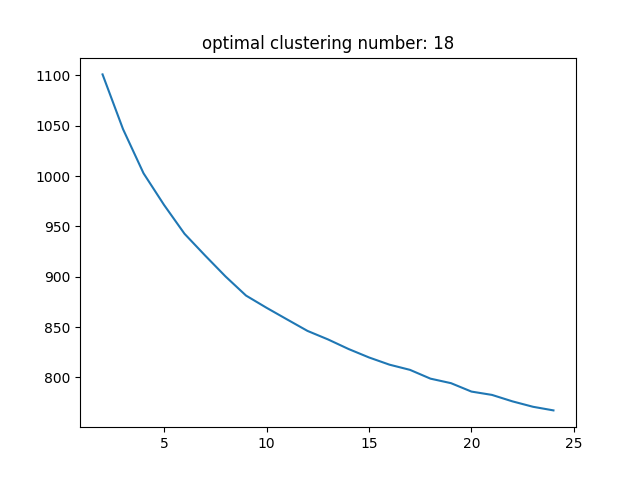
\includegraphics[width=1.0\textwidth]{elbow_method.png}}
    \caption{Elbow method for optimal clustering number}
    \label{elbow_method}
\end{figure}

為了要檢驗資料中的履歷是否與該申請之職缺相符,
我們使用了k-means\cite{macqueen1967some}作為分群方法,
利用elbow method來取得最適分群數(Optimal clustering number),
其結果如圖.~\ref{elbow_method},
所得值為18,


\subsection{跨領域範本}

\section{結論}


\begin{acks}
    謝謝老師上課所教授之知識,使得我們能得以完成此次報告研究。
\end{acks}

\bibliographystyle{ACM-Reference-Format}
\bibliography{mybib}

\end{document}
\endinput
